% Options for packages loaded elsewhere
\PassOptionsToPackage{unicode}{hyperref}
\PassOptionsToPackage{hyphens}{url}
%
\documentclass[
  doc,floatsintext]{apa6}
\usepackage{amsmath,amssymb}
\usepackage{iftex}
\ifPDFTeX
  \usepackage[T1]{fontenc}
  \usepackage[utf8]{inputenc}
  \usepackage{textcomp} % provide euro and other symbols
\else % if luatex or xetex
  \usepackage{unicode-math} % this also loads fontspec
  \defaultfontfeatures{Scale=MatchLowercase}
  \defaultfontfeatures[\rmfamily]{Ligatures=TeX,Scale=1}
\fi
\usepackage{lmodern}
\ifPDFTeX\else
  % xetex/luatex font selection
\fi
% Use upquote if available, for straight quotes in verbatim environments
\IfFileExists{upquote.sty}{\usepackage{upquote}}{}
\IfFileExists{microtype.sty}{% use microtype if available
  \usepackage[]{microtype}
  \UseMicrotypeSet[protrusion]{basicmath} % disable protrusion for tt fonts
}{}
\makeatletter
\@ifundefined{KOMAClassName}{% if non-KOMA class
  \IfFileExists{parskip.sty}{%
    \usepackage{parskip}
  }{% else
    \setlength{\parindent}{0pt}
    \setlength{\parskip}{6pt plus 2pt minus 1pt}}
}{% if KOMA class
  \KOMAoptions{parskip=half}}
\makeatother
\usepackage{xcolor}
\usepackage{graphicx}
\makeatletter
\def\maxwidth{\ifdim\Gin@nat@width>\linewidth\linewidth\else\Gin@nat@width\fi}
\def\maxheight{\ifdim\Gin@nat@height>\textheight\textheight\else\Gin@nat@height\fi}
\makeatother
% Scale images if necessary, so that they will not overflow the page
% margins by default, and it is still possible to overwrite the defaults
% using explicit options in \includegraphics[width, height, ...]{}
\setkeys{Gin}{width=\maxwidth,height=\maxheight,keepaspectratio}
% Set default figure placement to htbp
\makeatletter
\def\fps@figure{htbp}
\makeatother
\setlength{\emergencystretch}{3em} % prevent overfull lines
\providecommand{\tightlist}{%
  \setlength{\itemsep}{0pt}\setlength{\parskip}{0pt}}
\setcounter{secnumdepth}{5}
% Make \paragraph and \subparagraph free-standing
\ifx\paragraph\undefined\else
  \let\oldparagraph\paragraph
  \renewcommand{\paragraph}[1]{\oldparagraph{#1}\mbox{}}
\fi
\ifx\subparagraph\undefined\else
  \let\oldsubparagraph\subparagraph
  \renewcommand{\subparagraph}[1]{\oldsubparagraph{#1}\mbox{}}
\fi
\ifLuaTeX
\usepackage[bidi=basic]{babel}
\else
\usepackage[bidi=default]{babel}
\fi
\babelprovide[main,import]{english}
% get rid of language-specific shorthands (see #6817):
\let\LanguageShortHands\languageshorthands
\def\languageshorthands#1{}
% Manuscript styling
\usepackage{upgreek}
\captionsetup{font=singlespacing,justification=justified}

% Table formatting
\usepackage{longtable}
\usepackage{lscape}
% \usepackage[counterclockwise]{rotating}   % Landscape page setup for large tables
\usepackage{multirow}		% Table styling
\usepackage{tabularx}		% Control Column width
\usepackage[flushleft]{threeparttable}	% Allows for three part tables with a specified notes section
\usepackage{threeparttablex}            % Lets threeparttable work with longtable

% Create new environments so endfloat can handle them
% \newenvironment{ltable}
%   {\begin{landscape}\centering\begin{threeparttable}}
%   {\end{threeparttable}\end{landscape}}
\newenvironment{lltable}{\begin{landscape}\centering\begin{ThreePartTable}}{\end{ThreePartTable}\end{landscape}}

% Enables adjusting longtable caption width to table width
% Solution found at http://golatex.de/longtable-mit-caption-so-breit-wie-die-tabelle-t15767.html
\makeatletter
\newcommand\LastLTentrywidth{1em}
\newlength\longtablewidth
\setlength{\longtablewidth}{1in}
\newcommand{\getlongtablewidth}{\begingroup \ifcsname LT@\roman{LT@tables}\endcsname \global\longtablewidth=0pt \renewcommand{\LT@entry}[2]{\global\advance\longtablewidth by ##2\relax\gdef\LastLTentrywidth{##2}}\@nameuse{LT@\roman{LT@tables}} \fi \endgroup}

% \setlength{\parindent}{0.5in}
% \setlength{\parskip}{0pt plus 0pt minus 0pt}

% Overwrite redefinition of paragraph and subparagraph by the default LaTeX template
% See https://github.com/crsh/papaja/issues/292
\makeatletter
\renewcommand{\paragraph}{\@startsection{paragraph}{4}{\parindent}%
  {0\baselineskip \@plus 0.2ex \@minus 0.2ex}%
  {-1em}%
  {\normalfont\normalsize\bfseries\itshape\typesectitle}}

\renewcommand{\subparagraph}[1]{\@startsection{subparagraph}{5}{1em}%
  {0\baselineskip \@plus 0.2ex \@minus 0.2ex}%
  {-\z@\relax}%
  {\normalfont\normalsize\itshape\hspace{\parindent}{#1}\textit{\addperi}}{\relax}}
\makeatother

\makeatletter
\usepackage{etoolbox}
\patchcmd{\maketitle}
  {\section{\normalfont\normalsize\abstractname}}
  {\section*{\normalfont\normalsize\abstractname}}
  {}{\typeout{Failed to patch abstract.}}
\patchcmd{\maketitle}
  {\section{\protect\normalfont{\@title}}}
  {\section*{\protect\normalfont{\@title}}}
  {}{\typeout{Failed to patch title.}}
\makeatother

\usepackage{xpatch}
\makeatletter
\xapptocmd\appendix
  {\xapptocmd\section
    {\addcontentsline{toc}{section}{\appendixname\ifoneappendix\else~\theappendix\fi\\: #1}}
    {}{\InnerPatchFailed}%
  }
{}{\PatchFailed}
\keywords{papaja, APA}
\usepackage{csquotes}
\usepackage[backend=biber,style=apa]{biblatex}
\DeclareLanguageMapping{german}{german-apa}
\addbibresource{lit.bib}
\DefineBibliographyStrings{ngerman}{references = {Literaturverzeichnis}}
\usepackage{times}
\babelprovide[main,import]{ngerman}
\usepackage{floatrow}
\floatsetup[figure]{capposition=top}
\floatsetup[table]{capposition=top}
\ifLuaTeX
  \usepackage{selnolig}  % disable illegal ligatures
\fi
\usepackage[]{biblatex}
\IfFileExists{bookmark.sty}{\usepackage{bookmark}}{\usepackage{hyperref}}
\IfFileExists{xurl.sty}{\usepackage{xurl}}{} % add URL line breaks if available
\urlstyle{same}
\hypersetup{
  pdftitle={APA und die deutsche Sprache},
  pdfauthor={Prof.~Dr.~Stephan Huber1,2},
  pdflang={en-EN},
  pdfkeywords={papaja, APA},
  hidelinks,
  pdfcreator={LaTeX via pandoc}}

\title{APA und die deutsche Sprache}
\author{Prof.~Dr.~Stephan Huber\textsuperscript{1,2}}
\date{}


\shorttitle{APA und die deutsche Sprache}

\authornote{

Alle Dateien im Zusammenhang mit diesem Document findet man hier: \url{https://github.com/hubchev/ewa}. Kontakt bitte über \texttt{stephan.huber@hs-fresenius.de} aufnehmen.

}

\affiliation{\vspace{0.5cm}\textsuperscript{1} Fresenius University of Applied Science\\\textsuperscript{2} Charlotte Fresenius University}

\abstract{%
In diesem Dokument zeige ich wie ein APA konformes Manusskript erstellt werden kann. Hierzu passe ich die Vorlage des `papaja' packages \autocite{R-papaja} an.
}



\begin{document}
\maketitle

\hypertarget{apa-papaja-und-die-deutsche-sprache}{%
\section{\texorpdfstring{APA, \texttt{papaja} und die deutsche Sprache}{APA, papaja und die deutsche Sprache}}\label{apa-papaja-und-die-deutsche-sprache}}

Das \texttt{papaja} package von \textcite{R-papaja} erlaubt das Erstellen von APA konformen Manuskripten mit R Markdown. Die \texttt{papaja} Vorlage ist für die englische Sprache konzipiert. Will man nun in deutscher Sprache publizieren muss hier einiges angepasst werden. Ich werde im Folgenden zeigen, wie das geht. Zuvor sollte aber die Frage gestellt werden, ob die APA Formatierungs und Zietierregeln überhaupt für eine deutschsprachige Publikation eingefordert werden können. Die Regeln werden von der \textcite{Association2020Publication} festgelegt und setzen die Richtlinien naturgemäß für die englische Sprache. Eine offizielle Übersetzung der englischen APA-Richtlinien gibt es nicht. Anstatt dessen braut jeder so ein bisschen sein Süppchen. Viele Dozenten und (deutsche) Universitäten verweisen in ihren ``Handbüchern zum verfassen von Abschlussarbeiten'' auf APA, bleiben aber genauere Angaben schuldig. Leider lassen sich nicht ohne weitere Bestimmungen und Übersetzungsregeln übertragen. Eine Rücksprache mit dem Verlag, dem Auftraggeber, oder der Universität ist hier zwingend erforderlich. Beispielsweise sollte geklärt werden ob konsistent die deutsche oder die englischen Bezeichnungen verwendet werden sollen (beispielsweise ``Herausgeber'' vs.~``Editor'' oder ``Band'' vs.~``Volume''). Ich empfehle hier die englische Bezeichnungen zu wählen, wenn die Mehrzahl der Referenzen in englischer Sprache sind.

\hypertarget{warum-deutsch}{%
\section{Warum Deutsch?}\label{warum-deutsch}}

Englisch ist anerkannte Wissenschaftssprache und sollte für die Verbreitung von Wissen die erste Wahl sein. Durch die Wahl der deutschen Sprache, wird der Zugang unnötig erschwert. Ich sehe folgende Gründe, für eine Publikation in deutscher Sprache:

\begin{enumerate}
\def\labelenumi{\arabic{enumi}.}
\tightlist
\item
  Die Autoren können kein Englisch.
\item
  Der Verlag will Deutsch als Wissenschaftssprache fördern.
\item
  Der Verlag ist für die weltweite Vermarktung betriebswirtschaftlich nicht ausgelegt.
\item
  Es wird eine zügige und große Verbreitung im deutschsprachigen Raum angestrebt.
\item
  Die Inhalte der Arbeit sind besonders von regionalem Interesse.
\item
  Die Arbeit will im deutschsprachigen Raum insbesondere von populärwissenschaftliche Kreise beachtet werden.
\end{enumerate}

\hypertarget{anpassungen-an-der-papaja-vorlage}{%
\section{\texorpdfstring{Anpassungen an der \texttt{papaja} Vorlage}{Anpassungen an der papaja Vorlage}}\label{anpassungen-an-der-papaja-vorlage}}

Eine Anpassung der \texttt{papaja} Vorlage bedingt etwas Wissen über \LaTeX\footnote{\LaTeX~ist ein plattformunabhängiges und freies Softwarepaket. Anders als beispielsweise das Textverarbeitungsprogramm MS Word funktioniert \LaTeX~nicht nach dem ``What-you-see-is-what-you-get''-Prinzip. Anstatt dessen wird ausschließlich mit Text und Makros gearbeitet, um das Erscheinungsbild der Publikation zu manipulieren. Besonders in Wissenschaftsverlagen findet es Anwendung. So wird praktisch alles bei Springer oder Elsevier mit \LaTeX~gesetzt.}. Dies ist für die Erstellung der pdf Datei verantwortlich.

Ich identifiziere im Wesentlichen folgenden Anpassungsbedarf in \texttt{papaja}\footnote{Sollten weitere Sachen auffallen, werde ich gerne versuchen diese zu behandeln.}:

\begin{enumerate}
\def\labelenumi{\arabic{enumi}.}
\tightlist
\item
  Einige Übersetzungen, wie ``Table'', ``Figure'', ``Note'', ``Table of Contents'' und ``Literature''.
\item
  Entsprechend APA Version 7 müssen auch für Abbildungen die Überschriften oberhalb der Abbildung gesetzt werden, siehe: \url{https://apastyle.apa.org/style-grammar-guidelines/tables-figures/figures}.
\item
  Die Schriftart in \emph{Times New Roman} verändern.\footnote{Voreingestellt ist die Schriftart Computer Modern. Das ist APA konform.}
\item
  Die Autoren werden mit ``and'' verbunden. Hier sollte aber das deutsche ``und'' stehen, oder ``\&''.
\item
  Einfügen eines Appendix nach dem Literaturverzeichnis.
\end{enumerate}

Um 1., 2. und 3. einzuarbeiten, sollte dem YAML header Folgendes hinzugefügt werden:

\begin{verbatim}
  header-includes:
    - \usepackage{times}
    - \babelprovide[main,import]{ngerman}
    - \usepackage{floatrow}
    - \floatsetup[figure]{capposition=top}
    - \floatsetup[table]{capposition=top}
  ---
\end{verbatim}

Zusätzlich sollte noch Folgendes gleich unterhalb des YAML header geschrieben werden:

\begin{verbatim}
```{r}
de_terms <- getOption("papaja.terms")
de_terms$note <- "Anmerkungen"
de_terms$keywords <- "Schlüsselbegriffe"
options("papaja.terms" = de_terms) 
rm(list = ls())
```
\end{verbatim}

Punkt 4. zu berücksichtigen, ist etwas problematischer: APA ist schlicht kein deutscher Zitierstil und beid er gleichzietigen Zitation von deutschsprachiger und englischsprachiger Literatur sind Kompromisse unumgänglich.
Es gibt unzählige Zitierstile die auf APA angelehnt sind. Hier eine Liste: \url{https://www.zotero.org/styles?q=apa}.
Ich schlage vor, einen dieser Zitierstile zu verwenden:

\begin{itemize}
\tightlist
\item
  \url{https://www.zotero.org/styles/apa}: Hier handelt es sich um den APA Version 7 Zitierstil, wobei mit dem \emph{ampersand} (``\&'') anstatt dem \emph{and} gearbeitet wird.
\item
  \url{https://www.zotero.org/styles/deutsche-gesellschaft-fur-psychologie}: Hier handelt es sich um den Zitierstil \emph{Deutsche Gesellschaft für Psychologie 5. Auflage (Deutsch)}.
\end{itemize}

Den gewünschten Stil runterladen und Folgendes in den YAML header aufnehmen:

\begin{verbatim}
csl               : "apa.csl"
\end{verbatim}

Eine Sache sollte noch angepasst werden. Anstatt ``and'' sollte jetzt ``und'' zwischen den Autoren stehen, wenn diese zitiert werden. Dies gelingt durch Folgendes im YAML header:

\begin{verbatim}
output            : 
  papaja::apa6_pdf:
    citation_package: biblatex

csl               : "apa.csl"
header-includes:
  - \usepackage[backend=biber,style=apa]{biblatex} 
  - \DeclareLanguageMapping{german}{german-apa}
  - \addbibresource{lit.bib}
  - \DefineBibliographyStrings{ngerman}{references = {Literaturverzeichnis}}
\end{verbatim}

Sowie der Befehl das Literaturverzeichnis auch zu setzen. Dies sollte derart geschehen:\footnote{Darüber hinaus muss sichergestellt sein, dass auf dem entsprechenden PC \texttt{biber} installiert ist. In Debian geschieht dies etwa durch \texttt{sudo\ apt\ install\ biber} und in MAC durch \texttt{brew\ install\ biber}. In der Posit Cloud läuft es ohne Probleme und ohne extra Installation.}

\begin{verbatim}
\printbibliography
\end{verbatim}

Um 5. umzusetzen, sollte am Ende der eigentlichen .Rmd Datei dies hier eingefügt werden:

\begin{verbatim}
\newpage
# (APPENDIX) Appendix {-} 
\end{verbatim}

\hypertarget{empfehlungen}{%
\section{Empfehlungen}\label{empfehlungen}}

Anstatt die einzelnen Teile manuell in den YAML header und den Text einzufügen, empfehle ich das github repository zu klonen beziehungweise zu herunterzuladen und die entsprechende .Rmd Datei als Vorlage zu verwenden. Der YAML header ist außerordentlich empfindlich. Ein Leerzeichen zuviel und nichts funktioniert.

Darüber hinaus bitte ich möglichst wenig von der Vorlage abzuweichen. Fast alle Änderungswünsche von Studierenden die ich bislang miterleben durfte, stellen keine Verbesserung dar. Schlichtheit ist trumpf bei wissenschaftlichen Arbeiten. Insbesondere Verlage, Herausgeber und wissenschaftliche Gutachter (Professoren, Referees, Kursleiter) sind über wenig verschnörkselte Manuskripte dankbar.

\printbibliography
\clearpage

\newpage

\hypertarget{appendix-appendix}{%
\appendix}


\hypertarget{das-ist-der-erste-anhang}{%
\section{Das ist der erste Anhang}\label{das-ist-der-erste-anhang}}

Hier befindet sich Abbildung \ref{fig:plotcar} sowie Tabelle \ref{tab:mixedtab}.

\clearpage

\begin{figure}
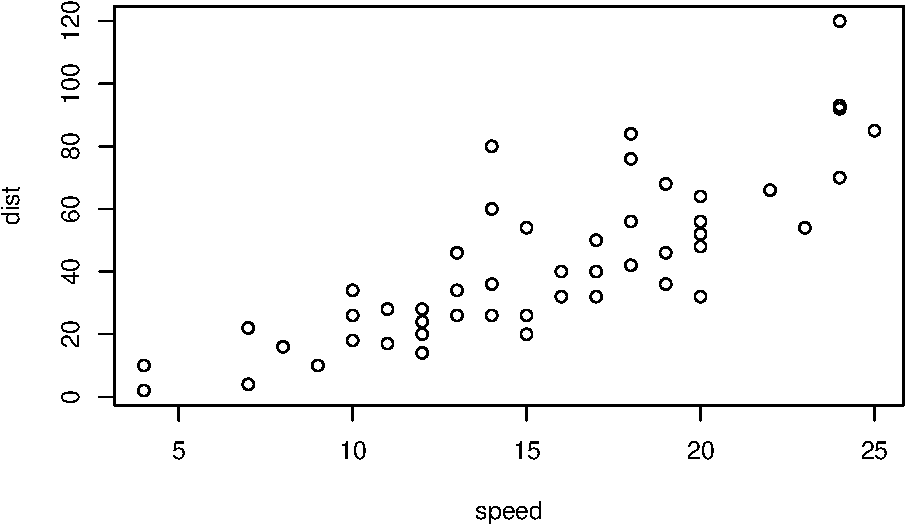
\includegraphics[width=\textwidth]{rmd_apa_deutsch_files/figure-latex/plotcar-1} \caption{Das ist ein gaaaaaaaaaaaaaaaaaaaaaaaaaaaaaaaaaaannnnnnnzzzz lange Überschrift für eine Abbildung.}\label{fig:plotcar}
\end{figure}

\begin{table}[tbp]

\begin{center}
\begin{threeparttable}

\caption{\label{tab:mixedtab}Descriptive statistics of correct recall by dosage.}

\begin{tabular}{llllll}
\toprule
Dosage & \multicolumn{1}{c}{Mean} & \multicolumn{1}{c}{Median} & \multicolumn{1}{c}{SD} & \multicolumn{1}{c}{Min} & \multicolumn{1}{c}{Max}\\
\midrule
A & 14.19 & 14.00 & 4.45 & 5 & 25\\
B & 13.50 & 14.00 & 5.15 & 4 & 22\\
C & 19.19 & 19.00 & 3.52 & 13 & 25\\
\bottomrule
\addlinespace
\end{tabular}

\begin{tablenotes}[para]
\normalsize{\textit{Anmerkungen.} This table was created with apa\_table().}
\end{tablenotes}

\end{threeparttable}
\end{center}

\end{table}

\newpage

\hypertarget{der-yaml-header-ist-ein-weiterer-anhang}{%
\section{Der YAML Header ist ein weiterer Anhang}\label{der-yaml-header-ist-ein-weiterer-anhang}}

\begin{verbatim}
---
title             : "APA und die deutsche Sprache"
shorttitle        : "APA und die deutsche Sprache"

author: 
  - name          : "Prof. Dr. Stephan Huber"
    affiliation   : "1,2"
    corresponding : no    # Define only one corresponding author
    address       : "Im Mediapark 4e"
    email         : "stephan.huber@hs-fresenius.de"

affiliation:
  - id            : "1"
    institution   : "Fresenius University of Applied Science"
  - id            : "2"
    institution   : "Charlotte Fresenius University"

authornote: |
  Alle Dateien im Zusammenhang mit diesem Document findet man hier: [https://github.com/hubchev/ewa](https://github.com/hubchev/ewa). Kontakt bitte über `stephan.huber@hs-fresenius.de` aufnehmen.

abstract: |
  In diesem Dokument zeige ich wie ein APA konformes Manusskript erstellt werden kann. Hierzu passe ich die Vorlage des 'papaja' packages [@R-papaja] an.

keywords          : "papaja, APA"

floatsintext      : yes
linenumbers       : no
draft             : no
mask              : no
numbersections    : yes

figurelist        : yes
tablelist         : yes
footnotelist      : no

classoption       : "doc"
toc               : yes

output            : 
  papaja::apa6_pdf:
    citation_package: biblatex

csl               : "apa.csl"
header-includes:
  - \usepackage[backend=biber,style=apa]{biblatex} 
  - \DeclareLanguageMapping{german}{german-apa}
  - \addbibresource{lit.bib}
  - \DefineBibliographyStrings{ngerman}{references = {Literaturverzeichnis}}
  - \usepackage{times}
  - \babelprovide[main,import]{ngerman}
  - \usepackage{floatrow}
  - \floatsetup[figure]{capposition=top}
  - \floatsetup[table]{capposition=top}
---
\end{verbatim}


\printbibliography

\end{document}
